\renewcommand{\theequation}{\theenumi}
\begin{enumerate}[label=\thesubsection.\arabic*.,ref=\thesubsection.\theenumi]
\numberwithin{equation}{enumi}

%\item An apache helicopter of the enemy is flying along the curve given by 
%	\label{prob:dist_pt_parab_sdp}
%\begin{align}
%\label{eq:dist_pt_parab_sdp}
%y = x^2 +7
%\end{align}
%%
%A soldier, placed at 
%\begin{align}
%\vec{P} = \myvec{3\\7}.  
%\end{align}
%%
%wants to shoot the heicopter when it is nearest to him.  Express this as an optimization problem.
\item
	\label{prob:dist_pt_parab_sdp}
Express the problem of 
finding the point on the curve 
\begin{align}
\label{eq:dist_pt_parab_sdp}
x^2 = 2y
\end{align}
%
nearest to the point 
\begin{align}
\vec{P} = \myvec{0\\5}.  
\end{align}
%
as an optimization problem.
\\
\solution The given problem can be expressed as
%
\begin{align}
\label{eq:qp_dist_pt_parab_sdp_qp}
\min_{\vec{x}}\vec{x}^T\vec{Q}_0\vec{x}+\vec{q}_0^T\vec{x}+c_0
\\
\text{s.t. }\vec{x}^T\vec{Q}_1\vec{x} + \vec{q}_1^T\vec{x} +c_1 \le 0
\end{align}
%
%where $\vec{V} \succeq 0$.
%\begin{align}
%\label{eq:qp_dist_pt_parab_sdp}
%\begin{split}
%\min_{\vec{x}}\vec{X}^T\myvec{\vec{I} & \vec{0} \\ \vec{0} & \vec{0}}\vec{X}-2\myvec{\vec{P}^T & \vec{0}}\vec{X}+\norm{\vec{P}}^2
%\\
%\text{s.t. }\vec{x}^T\vec{V}\vec{x} + \vec{u}^T\vec{x}  = 0
%\end{split}
%\end{align}
%
where
%
\begin{align}
\vec{Q}_0 &= \vec{I}, \vec{Q}_1 = \myvec{1 & 0\\0 & 0}
\\
\vec{q}_0 &=-2\vec{P}, \vec{q}_1 = -2\myvec{0 \\ 1}
\\
c_0 &= \norm{\vec{P}}^2, c_1 = 0
\end{align}
%\item Show that the constraint in 	
%%\label{prob:dist_pt_parab_sdp}
%\eqref{eq:qp_dist_pt_parab_sdp} is nonconvex.
%
\item Show that \eqref{eq:qp_dist_pt_parab_sdp_qp} is equivalent to
\begin{align}
\label{eq:qp_dist_pt_parab_sdp_conv}
\begin{split}
\min_{\vec{x},\theta}\theta
\\
\text{s.t. } \myvec{\vec{I} & \vec{M}_0\vec{x} \\ \vec{x}^T\vec{M}_0^T & -c_0-q_0^T\vec{x}+\theta} &\succeq 0
\\
\myvec{\vec{I} & \vec{M}_1\vec{x} \\ \vec{x}^T\vec{M}_1^T & -c_1-q_1^T\vec{x}} &\succeq 0
\end{split}
\end{align}
%
%\item Show that the following {\em relaxation} makes \eqref{eq:qp_dist_pt_parab_sdp} a convex optimization problem.
%%
%\begin{align}
%\label{eq:qp_dist_pt_parab_sdp_conv}
%\min_{\vec{x}}\brak{\vec{x}-\vec{P}}^T\brak{\vec{x}-\vec{P}}
%\\
%\text{s.t. }\vec{x}^T\vec{V}\vec{x} + \vec{u}^T\vec{x}  \le 0
%\end{align}
%
where
\begin{align}
\vec{Q}_i = \vec{M}_i^T\vec{M}_i, i = 0, 1
\end{align}
%
\item Solve \eqref{eq:qp_dist_pt_parab_sdp_conv} using cvxpy.
\item Graphically verify the solution to Problem \ref{prob:dist_pt_parab_sdp}. 
%\\
%\solution  The following code yields the minimum distance as 2.236 and the nearest point on the curve as
%%
%\begin{align}
%\vec{Q} &= \myvec{1\\8}
%\end{align}
%
%\begin{lstlisting}
%codes/opt/qp_cvx.py
%\end{lstlisting}

\item Solve \eqref{eq:qp_dist_pt_parab_sdp_qp} using the method of Lagrange multipliers.
%by drawing a figure.
%\\
%\solution 
%The following code plots Fig. \label{fig:qp_parab_sdp}
%%	
%\begin{lstlisting}
%codes/opt/qp_parab.py
%\end{lstlisting}
%
%%
%\begin{figure}[!ht]
%\centering
%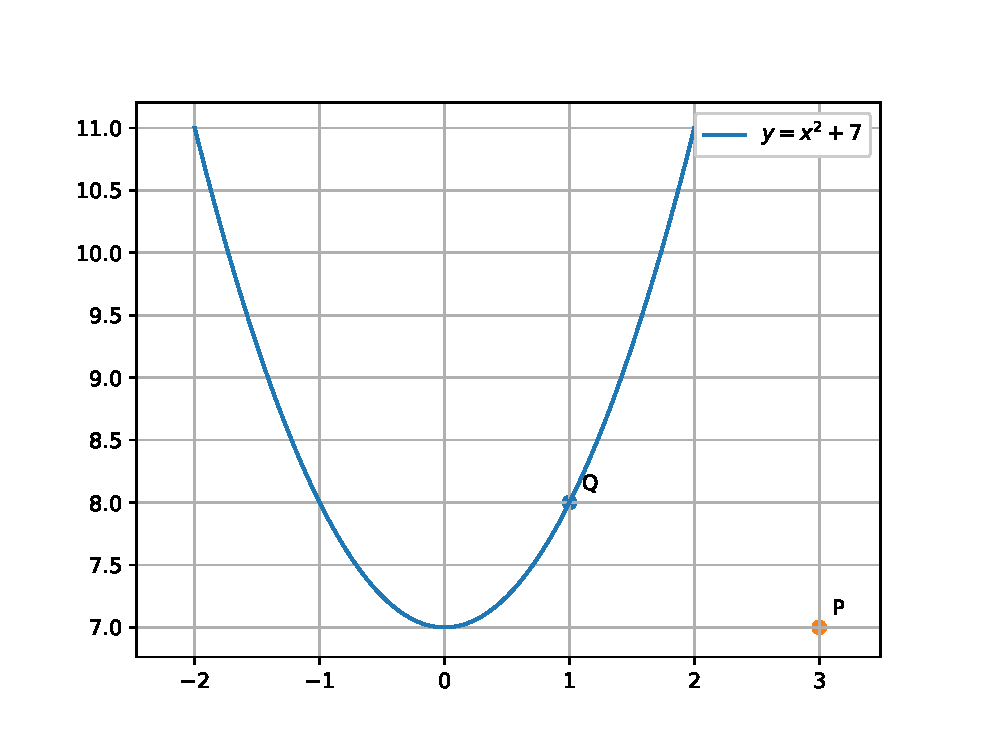
\includegraphics[width=\columnwidth]{./figs/opt/qp_parab.eps}
%\caption{ $\vec{Q}$ is closest to $\vec{P}$}.
%\label{fig:qp_parab_sdp}
%\end{figure}
%
%\item Frame 	
% as an optimization problem.
%\label{prob:qp_dist_pt_parab}
%\\
%
%\solution 
%From \eqref{eq2_1_line} and \eqref{eq2_1_circ}, 
%%
%\begin{align}
%r^2 & = (x_1-8)^2 + (3- x_1)^2 \\
%&= 2 x_1^2 - 22 x_1 + 73 \\
%\Rightarrow r^2 &= \frac{\brak{2x_1-11}^2 + 5^2}{2}
%\end{align}
%%
%which is minium when $x_1 = \frac{11}{2}, x_2 = \frac{7}{2}$.  The minimum value is $\frac{25}{2}$ and 
%the radius $r = \frac{5}{\sqrt{2}}$.
%	
%\begin{lstlisting}
%codes/opt/optimization/lagmul.py
%\end{lstlisting}
%\item Solve \eqref{eq:qp_dist_pt_parab_sdp_conv} using gradient descent.
%
\end{enumerate}
